%%%%%%%%%%%%%%%%%%%%%%%%%%%%%%%%%%%%%%%%%%%%%%%%%%%%%%%%%%%%%%%%%%%%%
%
%  This is a sample LaTeX input file for your contribution to
%  the MC2013 conference. Modified by R.C. Martineau at INL from A.
%  Sood at LANL, from J. Wagner ORNL who obtained the original class
%  file by Jim Warsa, LANL, 16 July 2002}
%
%  Please use it as a template for your full paper
%    Accompanying/related file(s) include:
%       1. Document class/format file: mc2013.cls
%       2. Sample Postscript Figure:   figure.eps
%       3. A PDF file showing the desired appearance: template.pdf
%    Direct questions about these files to: richard.martinea@inl.gov
%
%    Notes:
%      (1) You can use the "dvips" utility to convert .dvi
%          files to PostScript.  Then, use either Acrobat
%          Distiller or "ps2pdf" to convert to PDF format.
%      (2) Different versions of LaTeX have been observed to
%          shift the page down, causing improper margins.
%          If this occurs, adjust the "topmargin" value in the
%          mc2013.cls file to achieve the proper margins.
%
%%%%%%%%%%%%%%%%%%%%%%%%%%%%%%%%%%%%%%%%%%%%%%%%%%%%%%%%%%%%%%%%%%%%%


%%%%%%%%%%%%%%%%%%%%%%%%%%%%%%%%%%%%%%%%%%%%%%%%%%%%%%%%%%%%%%%%%%%%%
\documentclass{anstopical-class/ansconf}
%
%  various packages that you may wish to activate for usage
\usepackage{graphicx}
\usepackage{tabls}
\usepackage{multirow}
%
% my packages
\usepackage{amsmath} % math stuff
\usepackage{amssymb} % more math stuff
\usepackage{siunitx} % units and stuff
\sisetup{detect-weight=true, detect-family=true} % makes siunitx follow font formatting like bold, italic, etc.
\usepackage{cancel} % cancel stuff in eqns
\usepackage{isotope} % makes isotopes look pretty
\usepackage{listings} % makes code look pretty
\usepackage[dvipsnames,table]{xcolor} % colors
\usepackage{xspace} % space
\usepackage{booktabs} % table stuff
\usepackage{setspace} % more space
\usepackage{subcaption} % subfigure stuff
\usepackage{svg} % svg format figure stuff
\usepackage{hyperref} % makes refs good
\usepackage[final]{varioref} % makes refs even gooder
\usepackage{cleveref} % makes refs gooder
% adds oxford comma to cleveref
\newcommand{\creflastconjunction}{, and\nobreakspace}
\usepackage{lipsum} % lorem ipsum filler

% si units stuff
\DeclareSIUnit\year{yr}
\DeclareSIUnit\hour{hr}
\DeclareSIUnit\amp{A}

% check and x marks
\usepackage{pifont}% http://ctan.org/pkg/pifont
\newcommand{\cmark}{\textcolor{Green}{\ding{51}}}%
\newcommand{\xmark}{\textcolor{Red}{\ding{55}}}%
%
% Insert authors' names and short version of title in lines below
%
%\authorHead{Authors' names, use et al. if more than 3}
%\shortTitle{Short version of title as entered by author on web %page}

%\confTitle{19$^{th}$ International Conference on Nuclear Reactor %Thermal Hydraulics (NURETH-19)}
%\confLocation{Brussels, Belgium, August 29 -- September 3, 2021}

%Header and Page numbers

\usepackage{fancyhdr,graphicx,lastpage}% http://ctan.org/pkg/{fancyhdr,graphicx,lastpage}
\fancypagestyle{plain}{
\fancyhf{}
\fancyhead[L]{\begin{tabular}{ll}
\multirow{2}{*}{\includegraphics[scale=0.28]{anstopical-class/NURETH-19.png}} & \fontsize{9}{9}\selectfont {\setstretch{0.1}}The 19th International Topical Meeting on Nuclear Reactor Thermal Hydraulics (NURETH-19) Log nr.: 35861 \\
& \fontsize{9}{9}\selectfont Brussels, Belgium, March 6 - 11, 2022 \\
\end{tabular}} 
\fancyfoot[C]{\thepage}% Right footer
}



%%%%%%%%%%%%%%%%%%%%%%%%%%%%%%%%%%%%%%%%%%%%%%%%%%%%%%%%%%%%%%%%%%%%%
%
%   BEGIN DOCUMENT
%
%%%%%%%%%%%%%%%%%%%%%%%%%%%%%%%%%%%%%%%%%%%%%%%%%%%%%%%%%%%%%%%%%%%%%





\pagestyle{plain}% Set page style to plain.

\begin{document}

\title{EXPERIMENTS ON THE HELIUM-3 NEGATIVE REACTIVITY INSERTION (HENRI) PROTOTYPE AND FAST OPENING VALVE}

\author{A. Warren}
\author{A. Camargo}
\author{G. Mignot}
\author{W. Marcum}
\affil{School of Nuclear Science and Engineering \\
  Oregon State University, Corvallis, OR 97331 \\
  warrenau@oregonstate.edu; camargoa@oregonstate.edu}

%\author{Double space and list Author C}
%\affil{
%  Department of Nuclear Engineering \\
%  Name of University \\
%  Address \\
%  C@name.univ.edu
%}

\maketitle

\begin{abstract}
The restart of the Transient REactor Test (TREAT) facility combined with the Resumption of Transient Testing Program (RTTP) has generated an increased interest in mimicking Reactivity Initiated  Accident (RIA) events conditions for Light Water Reactor within TREAT itself. One of the engineering challenges for this task is to increase the energy deposition rate on the tested fuel element by shortening the width of the  power  pulse  from  its  current  89  milliseconds down  to  40 milliseconds. To overcome  this  challenge, Idaho National Laboratory (INL) proposed a design, consisting of rapidly pressurizing a specially designed hollow control rod with Helium-3. The insertion of negative reactivity in the form of Helium-3, a strong neutron  absorber,  must  be  well  predicted and repeatable.  In  this  prospect,  an  out-of-pile  prototype,  the Helium  Negative  Reactivity  Insertion  (HENRI) facility, has been designed  and  built  at  Oregon  State University (OSU) to  assess  the  feasibility,  the  repeatability, and  the control of such process. Tests performed with rupture disks provided characterization of the physics of the system, however the system requires a more repeatable and precise method of gas injection. To meet this need, a valve has been designed and tested using a pneumatic piston which can open rapidly and repeatedly for precise control of the system. These tests characterized the valve performance and provided confidence in the operation of the system, both of which are critical to understand and control the Helium-3 density evolution in the core.

\raggedleft
\textbf{KEYWORDS}\\
TREAT, Helium-3, Control Rod, Pulse, Valve
\end{abstract}


%\raggedright

%%%%%%%%%%%%%%%%%%%%%%%%%%%%%%%%%%%%%%%%%%%%%%%%%%%%%%%%%%%%%%%%%%%%%%%
%%%%%%%%%%%%%%%%%%%%%%%%%%% INTRODUCTION %%%%%%%%%%%%%%%%%%%%%%%%%%%%%%
%%%%%%%%%%%%%%%%%%%%%%%%%%%%%%%%%%%%%%%%%%%%%%%%%%%%%%%%%%%%%%%%%%%%%%%
% probably similar to previous HENRI NURETH intro
% motivations for TREAT RIA testing / HENRI project
% discuss the need for the fast opening piston valve -- maybe needs a different section?
\section{Introduction} \label{s:intro}
This section presents the background and motivations for the HENRI project, as well as the motivations and need for a fast-opening valve.

\subsection{HENRI Background} \label{ss:henri background}
% start with introduction / motivations of entire HENRI project
The Transient Reactor Test (TREAT) facility, located at the Materials and Fuels Complex at Idaho National Laboratory (INL), is a research reactor with the primary purpose of testing fuels under transient conditions and supporting the development of accident-tolerant fuel \cite{CINBIZ2017}. The reactor can shape these transients using control rods and the negative reactivity temperature feedback, with a maximum energy deposition of \SI{2500}{\mega\joule} \cite{Holschuh2019}. Currently, using only the temperature feedback of the reactor, the pulse full-width at half-maximum (FWHM) TREAT is capable of generating is around \SI{100}{\milli\second} \cite{Holschuh2019}. This pulse width is outside of the expected range for a Light Water Reactor (LWR) Reactivity Initiated Accident (RIA) of 30 to \SI{60}{\milli\second} \cite{NEA2010}. \Cref{fig:trans comp} presents a comparison of transient conditions that can be produced by contemporary reactors. There is not a reactor that can reproduce the conditions (FWHM and maximum power) of a LWR RIA. Using its control rods, TREAT can decrease its transient FWHM down to \SI{89}{\milli\second} \cite{NEA2010}, shown as a red dashed line in \Cref{fig:trans comp}. A further reduction in FWHM would bring TREAT near BWR conditions.



% transient reactor comparison plot -- ripped from source paper by Bess -- look for the one Mignot used in the old nureth paper
\begin{figure}[htbp]
    \vspace{16pt}
    \centering
    \includegraphics[width=0.75\textwidth]{intro/plots/ReactorTransientComp_Kevin.png}
    \caption{Comparison of contemporary reactor transient conditions \cite{BESS2019}.}
    \label{fig:trans comp}
    \vspace{16pt}
\end{figure}


In 1998, Crawford \cite{Crawford1998} suggested the use of helium-3, a strong neutron absorber gas, for clipping a high-power pulse in TREAT. Such a system would be capable of inserting a negative reactivity of -5\% $\Delta k/k$ without the use of control rods. The original calculation results in a FWHM reduced to 40-\SI{60}{\milli\second} for a total energy deposition of \SI{1600}{\mega\joule}, well below the \SI{2500}{\mega\joule} limit, and the peak power was estimated to be \SI{20000}{\mega\watt}. This pulse is more representative of the postulated LWR RIA and is shown as a red dotted line in \Cref{fig:trans comp}.

Helium-3 has been used for transient control at the CABRI reactor in Cadarache, France. At CABRI, helium-3 is pressurized in 4 tubes in the core, then to initiate a transient, the helium-3 is rapidly depressurized from the core, causing a positive reactivity insertion. This depressurization is precisely controlled using multiple valves to produce the desired pulse width and power for the transient \cite{Clamens2016,Clamens2018,Clamens2018b}. In TREAT, this process will be reversed by rapidly pressurizing tubes in the core with helium-3 to shut down a transient (negative reactivity insertion). CABRI has been updated and is currently used under the OECD/NEA CABRI International Project (CIP).

Initial calculations for the TREAT facility showed that a helium-3 pressure of \SI{1.72}{\mega\pascal} (\SI{250}{psi}) in four (4) cartridges, each with a volume of \SI{1167}{\centi\meter^3} would be sufficient to reach the desired negative reactivity of -5\% $\Delta k/k$. This pressure corresponds to an atomic density of \SI{3.35e20}{atoms\per\centi\meter^3}. For a pulse to be clipped properly, it is estimated that the helium-3 must be injected in \SI{5}{\milli\second} \cite{BESS2019}. Oregon State University (OSU) was tasked to model, design, and test an out-of-pile prototype cartridge to assess the feasibility and repeatability of the physical process; and identify and solve any engineering issues associated with the device. The experimental Helium-3 Negative Reactivity Insertion (HENRI) facility was designed and built at OSU. The previous work on HENRI used rupture disks to investigate if the desired pressurization speed was achievable and repeatable, using a range of initial pressures and rupture disk (orifice) sizes \cite{HeNURETH}. The largest tested orifice size, \SI{2.54}{\centi\meter} (1 inch) diameter, was selected to provide the highest flow rate; and TREAT would like to have flexibility in the initial pressure to shape transients to match various conditions, however, the optimal pressure range is 1.72-3.44 \si{\mega\pascal} (250-500 psi).



% describe the need for a new fast-opening valve -- should this be its own section?
\subsection{Need for a Fast-opening Valve} \label{ss:need for valve}

% The previous work on HENRI at OSU \cite{HeNURETH} used rupture disks to characterize the system and its physics. Rupture disks provided an almost instantaneous opening, which allowed for the gas physics to be isolated and compared against CFD models \cite{CFDNureth}. The rupture disks, however, have major drawbacks for use in the HENRI system for TREAT. Firstly, the rupture disks must be changed after each use, which would mean taking the HENRI system out of the TREAT reactor and dealing with the radiation of the system before changing the rupture disk and reinstalling the system in the reactor. This process adds danger and complexity, on top of the time, to a system intended to be utilized heavily during RIA testing campaigns. Secondly, the rupture disks do not rupture in a predictable manner. There is tolerance in the manufacture of rupture disks that causes the disks to rupture at slightly different pressures, which is not ideal when the system needs to be precisely timed with the peak of a transient. These problems with the rupture disk have lead OSU to investigate a more permanent valve option. This valve must be reusable, precise, fast-opening, and durable. The valve must also fit into the physical space constraints of the HENRI system, which includes its power or actuation method, and not contaminate the helium-3 used in the system.

The rupture disk tests provided good data to characterize the gas injection in the HENRI cartridge, however, the rupture disks can not be used for the final design since they are not reusable and they are not precise in their operation from disk to disk. Using rupture disks at TREAT would require cartridge removal between each test, which would significantly slow down the testing process. It was also found that the rupture disks had some variation in actual burst pressure for a stamped burst pressure, which causes the helium injection to be unpredictable. Therefore, an ideal valve must:
\begin{enumerate}
    \item open fast enough for the desired pressurization to occur in less than \SI{5}{\milli\second},
    \item open fully with no restrictions to flow,
    \item produce the same injection repeatedly,
    \item be operated without maintenance or replacement for multiple tests,
    \item be precisely triggered with a TREAT transient,
    \item fit in the physical confines of the HENRI cartridge in TREAT, and
    \item operate at a range of pressures, including low pressure (around or below \SI{1.72}{\mega\pascal}).
\end{enumerate}

These requirements are listed in \Cref{tab:valve comp}, where the rupture disks and various off-the-shelf valves are compared to the ideal valve. There is not an available commercial valve to meet the needs of the HENRI system, therefore, OSU has been tasked with designing and testing a bespoke valve for the system. This paper discusses  the valve design; the experimental setup and methodology used to test the valve; the experimental results; and the impact of the work.

% Table generated by Excel2LaTeX from sheet 'Sheet1'
\begin{table}[htbp]
  \centering
  \caption{Comparison of valves to ideal requirements.}
    \begin{tabular}{cccccccc}
    \toprule
    \textbf{Valve} & \textbf{Speed} & \textbf{Fully Open} & \textbf{Repeatable} & \textbf{Durable} & \textbf{Precise} & \textbf{Size} & \textbf{Low Pressure} \\
    \midrule
    \rowcolor[rgb]{ .851,  .851,  .851} Rupture Disk & \cmark   & \cmark   & \cmark   & \xmark    & \xmark    & \cmark   & \cmark \\
    Ball Valve & \xmark    & \xmark    & \cmark   & \cmark   & \cmark   & \xmark    & \cmark \\
    \rowcolor[rgb]{ .851,  .851,  .851} Needle Valve & \xmark    & \xmark    & \cmark   & \cmark   & \cmark   & \xmark    & \cmark \\
    Solenoid Valve & \cmark   & \cmark   & \cmark   & \cmark   & \cmark   & \xmark    & \cmark \\
    \rowcolor[rgb]{ .851,  .851,  .851} Ideal Valve & \cmark   & \cmark   & \cmark   & \cmark   & \cmark   & \cmark   & \cmark \\
    \bottomrule
    \end{tabular}%
  \label{tab:valve comp}%
\end{table}%



%\clearpage
%%%%%%%%%%%%%%%%%%%%%%%%%%%%%%%%%%%%%%%%%%%%%%%%%%%%%%%%%%%%%%%%%%%%%%%
%%%%%%%%%%%%%%%%%%%%%%%%%%%%%% DESIGN %%%%%%%%%%%%%%%%%%%%%%%%%%%%%%%%%
%%%%%%%%%%%%%%%%%%%%%%%%%%%%%%%%%%%%%%%%%%%%%%%%%%%%%%%%%%%%%%%%%%%%%%%
% discuss design requirements of fast opening valve -- why piston valve; why does burst disk not work
% discuss design iterations of piston valve -- first mount / metal-metal seal, then improved mount, and o-ring on plug
\section{Fast-Opening Valve Design} \label{s:design}
% talk about design requirements
% discuss the initial piston valve design -- what was it, how well did it work, why did it not work


To meet the requirements outlined above, a piston actuated valve was designed, built, and tested at OSU.
The valve utilizes the helium from the high pressure driver tank in HENRI as its working fluid, which decreases the chances of contamination compared to using another working fluid, as well as keeping the required external attachments to a minimum to improve the modularity of the HENRI cartridge.
The piston can fit inside the driver tank and attaches to the driver tank's flange.
The flange is machined to accept a machined plug that attaches to the piston to create a tight seal.
The valve can open rapidly by using the pressure of the helium in the driver tank and fully pulls away from the flange to provide obstruction-free flow into the test section.
\Cref{fig:cad gen 1} shows CAD models of the piston valve, both a concept model and an as-built model.
\Cref{fig:cad concept} shows the concept of the valve and how it attaches to the driver tank flange to sit inside the HENRI cartridge and \Cref{fig:cad lip} shows the as-built piston mount and flange.
The sealing surface has a lip machined into it that helps the metal plug to seal against the surface of the flange.

% obviously put a drawing and/or picture here of the og design -- also include a picture of the whole HENRI assembly with labels, so this all makes sense
\begin{figure}[b!]
    \vspace{16pt}
    \centering
    \begin{subfigure}[t]{0.6\textwidth}
        \centering
        \includegraphics[width=0.8\textwidth]{design/photos/PistonValve_Gen1_CAD_labels.PNG}
        \caption{CAD model of a piston valve concept attached to driver tank flange.}
        \label{fig:cad concept}
    \end{subfigure}
    \hfill
    \begin{subfigure}[t]{0.35\textwidth}
        \centering
        \includegraphics[width=0.8\textwidth]{design/photos/PistonMount_CAD_lip.PNG}
        \caption{As-built CAD model of first piston valve mount and driver tank flange, with sealing lip highlighted.}
        \label{fig:cad lip}
    \end{subfigure}
    \caption{CAD models of the piston valve with important features highlighted.}
    \label{fig:cad gen 1}
    \vspace{16pt}
\end{figure}

% should we talk about opening speed characterization? if so, we need plots / tables of results and maybe some pics of the set up

% The first plug design was made with various materials, including aluminum, stainless steel, and a cobalt alloy, seen in \Cref{fig:metal plugs}. This plug is a simple design with a \SI{45}{\degree} cone that directly contacts the matching machined surface of the flange. A special coating was also tried on an aluminum plug[DO WE HAVE THE COATING INFO?] to improve the sealing ability of the plug on the flange. The initial mount design for the piston was made of a plate mounted to the piston body and three legs holding the plate onto the flange. The three-legged design allowed for easy routing of tubing for operating the piston, but also allowed for some movement of the mount when the piston was fully extended. This movement caused asymmetric wear on the plug, as seen in \Cref{fig:metal plugs}, leading to failure of the seal. Potentially due to this wear, the slow flow through the manifold, or the nature of metal-to-metal seals, a slight leak was observed from the driver tank into the test section before the piston valve opened fully [REF to plot here?].

\begin{figure}[bt]
    \vspace{16pt}
    \centering
    \begin{subfigure}[t]{0.6\textwidth}
        \centering
        \includegraphics[width=0.7\textwidth]{design/photos/plug_gen1_drawing.PNG}
        \caption{Drawing of plug for piston valve. Measurements are in inches.}
        \label{fig:plug draw}
    \end{subfigure}
    \hfill
    \begin{subfigure}[t]{0.35\textwidth}
        \centering
        \includegraphics[width=0.58\textwidth]{design/photos/cobalt_plug.png}
        \caption{As-built plug for piston valve.}
        \label{fig:cobalt plug}
    \end{subfigure}
    %
    \caption{Drawing and picture of plug used for piston valve.}
    \label{fig:plug}
    \vspace{16pt}
\end{figure}



The plug is machined with a slope of \SI{45}{\degree} to allow for maximum flow through the valve opening. The sealing surface of the flange is machined to match this slope, and when the piston presses the plug into the flange, the plug seals into the lip machined into the flange. \Cref{fig:plug} shows the drawing for the plug, as well as a plug as-built for the piston valve. To function properly, the plug must be designed such that the force from the pressure in the driver tank a) does not overwhelm the piston opening force and b) is able to hold the plug sealed without additional pressure in the piston. Sealing with only the pressure in the driver tank allows for the the piston chambers to be empty before the valve opens, which reduces resistance for the piston's movement and therefore maximizes the piston valve opening speed. The top and bottom chamber can be seen in \Cref{fig:piston valve}, which shows the piston valve installed on its mount on the flange. The first piston valve design mount uses three (3) legs to hold the piston onto the flange, which allows for tubing to go from the connections on the flange to the connections on the piston.





% discuss design improvements in second iteration in both the mount and the o-ring
% \subsection{Design Iteration} \label{s:iteration}
% While the first plug and mount design proved the concept of a piston valve will work for the HENRI system, the seal durability was low and the piston opening was not as smooth or as fast as desired. To improve the valve, a new plug was designed using an o-ring to improve the sealing ability, and a new mount was designed to provide a more uniform and sturdy hold on the piston. The new assembly can be seen in \Cref{fig:piston assembly}. The new plug still uses a \SI{45}{\degree} slope to mate to the existing flange, but it does not go to a point like the previous design. It has a dovetail groove machined into it, as seen in \Cref{fig:Dovetail Groove}, to hold the o-ring in place such that the o-ring presses into the machined surface of the flange to strongly seal the driver tank from the test section. Two types of o-ring materials have been tested: an FFKM o-ring manufactured by Marko Rubber and a nitrile o-ring manufactured by Parker. The new mount was designed to work with the existing flange, so it uses the same bolt holes and needs to align the piston with the same sealing surface. The mount is comprised of three aluminum pieces: a circular plate mounted to the bottom of the piston, a circular plate to hold the mount on the flange, and a cylindrical support holding the two plates together and keeping the piston at the correct distance from the sealing surface. The cylindrical support has slots machined into it to allow for gas flow, tube fitting connections on the piston, and access to the bolts that mount the assembly to the flange.




%%%%%%%%%%%%%%%%%%%%%%%%%%%%%%%%%%%%%%%%%%%%%%%%%%%%%%%%%%%%%%%%%%%%%%%
%%%%%%%%%%%%%%%%%%%%%%%%%%%% EXPERIMENT %%%%%%%%%%%%%%%%%%%%%%%%%%%%%%%
%%%%%%%%%%%%%%%%%%%%%%%%%%%%%%%%%%%%%%%%%%%%%%%%%%%%%%%%%%%%%%%%%%%%%%%
% discuss experimental set up, differences between this set up and the previous rupture disk set up
% discuss differences in piston valve iterations and why changes were made
% pictures and stuff
% maybe test matrix?
\section{Experimental Facility and Methodology} \label{s:experiment}

This section will describe the experimental facility, highlighting the modifications from the rupture disk experiments, and the methodology used to test the piston valve.

% talk about basic methodology of experiments and testing, introduce the structure of the section


% section for experimental facility, comparison of rupture disk and piston valve test set ups
\subsection{Experimental Facility} \label{s:facility}

% P&ID, photos, etc. of facility -- highlight differences between burst disk and piston
The main facility, seen in \Cref{fig:HENRI Facility}, is set up similarly to a shock tube, with a driver tank on the floor, an intermediate tube section, a test section, and a reflector section. The whole facility is upside-down to the HENRI cartridge orientation in the TREAT core. In the reactor, the driver tank will be above the core with the test section in the fuel. The reflector section will extend past the fuel to provide space for the gas reflection effects outside of the active region in the core. The intermediate section allows for the driver tank to be positioned above the reactor core while also decreasing the total required volume of helium-3 for the HENRI system. The facility is made using 304 stainless steel. The test section and reflector are pipe with a \SI{4.826}{\centi\meter} outer diameter and \SI{0.368}{\centi\meter} wall thickness (1.5 inch schedule 40 NPS); the intermediate section is \SI{3.175}{\centi\meter} (1.25 inch) outer diameter tubing with \SI{0.3175}{\centi\meter} ($0.125$ inch) wall thickness; and the driver tank is pipe with a \SI{16.8275}{\centi\meter} outer diameter and \SI{0.7112}{\centi\meter} wall thickness (6 inch schedule 40 NPS). The piston valve is attached to the top flange of the driver tank and hangs inside.

%
\begin{figure}[htbp]
    \vspace{16pt}
    \centering
    \begin{subfigure}[t]{0.6\textwidth}
        \centering
        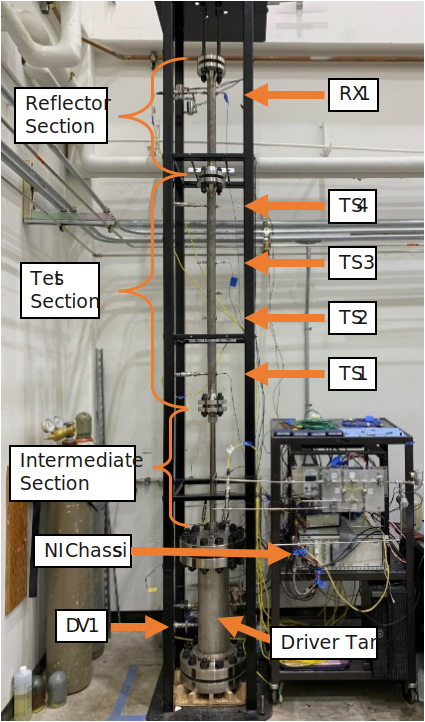
\includegraphics[width=2in]{experiment/photos/HENRI_labels.png}
        \caption{HENRI out-of-pile experimental facility.}
        \label{fig:HENRI Facility}
    \end{subfigure}
    \hfill
    \begin{subfigure}[t]{0.35\textwidth}
        \centering
        \includegraphics[width=0.9\textwidth]{design/photos/piston_mount_chambers.png}
        \caption{Piston valve attached to driver tank flange with mount, used for seal durability testing.}
        \label{fig:piston valve}
    \end{subfigure}
    \caption{HENRI experimental facility for piston valve testing.}
    \label{fig:facility}
    \vspace{16pt}
\end{figure}
%

The facility uses 13 pressure transducers and 1 thermocouple. The pressure transducers are one of two main types: Omega PX459 or PCB 113B24. All of the Omega pressure transducers are 0-1500 psia, except for two: a 0-3500 psia transducer used on the driver tank, and a 0-15 psia transducer used for the vacuum line. The Omega pressure transducers output a current from 4-\SI{20}{\milli\amp}, which is converted to voltage using a \SI{250}{\ohm} shunt resistor. The PCB transducers output a signal that is sent through a PCB Model 482C signal conditioner before being output to the voltage card. The data acquisition system uses a National Instruments (NI) PXIe-1085 chassis with a NI PXIe-8135 controller, a NI PXIe-4303 voltage input card for reading the instrumentation, and a NI PXI-6515 digital output card for controlling the solenoid valves. A piping and instrumentation diagram (P\&ID) for operating the piston valve can be seen in \Cref{fig:sv pid}. There is a manifold of four (4) solenoid valves used to operate the piston. SV-PI2 and SV-PI4 open to fill the top and bottom chamber, respectively; and SV-PI1 and SV-PI3 open to vent the top and bottom chamber, respectively. These solenoid valves are Parker Series 9 Miniature Calibrant Valve 009-0172-900. This particular valve was selected for its small form factor, high pressure rating, and low leak rate.

% %
% \begin{figure}[htbp]
%     \vspace{16pt}
%     \centering
%     \includegraphics[width=3.024in, height=4.032in]{experiment/photos/Piston_Assembly.jpg}
%     \caption{Piston assembled with second generation mount on flange.}
%     \label{fig:piston assembly}
%     \vspace{16pt}
% \end{figure}
% %


%
\begin{figure}[htbp]
    \vspace{16pt}
    \centering
    \includegraphics[width=0.6\textwidth]{experiment/photos/HENRI_valve_PID.PNG}
    \caption{Piping and instrumentation diagram (P\&ID) for piston valve operation.}
    \label{fig:sv pid}
    \vspace{16pt}
\end{figure}
%




% section for detailed experimental method (test matrix)
\subsection{Experimental Methodology} \label{s:methodology}

% we tested the plugs and o-rings for durability / sealing with sustained seal tests and repeated seal tests outside of the henri facility (just using the flange and piston)
% we tested the valve / plugs / o-rings in henri tests

The overall methodology for testing the piston valve includes two main parts: testing the plug designs for durability and sealing after large numbers of cycles; and testing the piston valve's performance in HENRI helium insertions. Testing the plugs was performed by cycling the piston valve to simulate the wear of long term use and comparing its sealing ability before and after the cycles. The LabVIEW code used for data acquisition was modified to automate the piston cycling process, so the plugs could be cycled overnight, then tested the next day to determine the seal degradation due to wear. This method was used for both the metal-to-metal seal plug and the o-ring plug. The valve's performance was tested by performing HENRI helium insertions at varying initial pressures to characterize the system's pressurization with the valve and compare the valve to the rupture disks.



%%%%%%%%%%%%%%%%%%%%%%%%%%%%%%%%%%%%%%%%%%%%%%%%%%%%%%%%%%%%%%%%%%%%%%%
%%%%%%%%%%%%%%%%%%%%%%%%%%%%% RESULTS %%%%%%%%%%%%%%%%%%%%%%%%%%%%%%%%%
%%%%%%%%%%%%%%%%%%%%%%%%%%%%%%%%%%%%%%%%%%%%%%%%%%%%%%%%%%%%%%%%%%%%%%%
% discuss / compare results to previous rupture disk stuff and previous iteration of piston valve
\section{Results and Discussion} \label{s:results}
This section will present the results of the work and discuss their significance. The piston valve is first compared to the previous results using the rupture disks to ensure the valve works as intended and provides the desired pressurization. The two piston valve iterations are compared to each other to see improvements; and the piston valve is compared to itself to determine reliability and consistency.

% subsection about piston v rupture disk
\subsection{Piston Valve Compared to Rupture Disk} \label{s:disk v piston}
The rupture disks were used in the HENRI system to determine if the system was capable of pressurizing to \SI{1724}{\kilo\pascal} (\SI{250}{psi}) in the desired time frame of \SI{5}{\milli\second}\cite{HeNURETH}. One of the goals of the piston valve is to open quickly enough to maintain as close to rupture disk physics as possible. 
%Computational fluid dynamics (CFD) simulations were validated using these experiments \cite{CFDNureth,HENRIATH}[MIGHT NEED DIFF REF HERE].
\Cref{fig:disk v piston} compares the results of a rupture disk test and a piston valve test, both with initial driver tank pressure of [PRESSURE] and intermediate tube diameter of \SI{2.54}{\centi\meter} (\SI{1}{inch}). [MORE discussion of the plot]

% plot goes here -- disk v piston
\begin{figure}[htbp]
    \vspace{16pt}
    \centering
    \includegraphics{}
    \caption{Comparison of rupture disk and piston valve HENRI tests at an initial pressure of [PRESSURE] and with intermediate tube diameter of \SI{2.54}{\centi\meter} (\SI{1}{inch}).}
    \label{fig:disk v piston}
    \vspace{16pt}
\end{figure}

The pressure evolution in the piston valve test follows what is expected from the rupture disk tests, which demonstrates the piston valve opens fast enough to meet the demands of the HENRI system. [MORE stuff specific to the plot] While a valve will not be as fast as a rupture disk due to needing a signal and having to actuate, this piston valve is fast enough and trades the small loss of speed for re-usability and predictability, which are strong improvements over the rupture disk. As described in \Cref{s:need for valve}, changing a rupture disk in between every test is not practical or feasible for the HENRI system in TREAT.


% first piston valve design
% the metal to metal seal did not last long -- durability issues, wear on the sealing surface, even with fancy materials; there was a small leak from the driver tank to the test section before the valve was fully open;

% subsection comparing metal-to-metal seal and o-ring plugs
\subsection{Metal-to-Metal Plug Compared to O-ring Plug}
The metal-to-metal plug design did not seal as well as the o-ring design, which led to a leak from the driver tank into the test section before the piston valve opened all the way. The o-ring plug does not have this issue, even at low operating pressures (below \SI{1.72}{\mega\pascal} (\SI{250}{psi})). \Cref{fig:metal vs oring} shows a test using each plug type. The pressure at [INSERT CORRECT POSITION HERE (probably TS1)] for the metal-to-metal seal increases slightly before the other positions, and before the driver tank pressure decreases significantly, showing that with only the pressure of the driver tank holding it closed, the metal-to-metal seal does not work well. In contrast, the o-ring plug is able to maintain the pressure boundary until the valve opens fully, which provides a quick, crisp helium injection.

\begin{figure}
    \vspace{16pt}
    \centering
    \includegraphics{}
    \caption{Results of tests with an initial pressure of [PRESSURE] for the metal-to-metal plug and the o-ring plug.}
    \label{fig:metal vs oring}
    \vspace{16pt}
\end{figure}

% subsection about predictability
\subsection{Piston Valve Predictability}
The piston valve's operation at a wide range of pressure must be characterized and predictable for the HENRI system's use in TREAT. The valve should be able to maintain its seal at low pressures, around \SI{1724}{\kilo\pascal} (\SI{250}{psi}), and the gas pressurization in the HENRI system must be determinable for any desired operating pressure. \Cref{fig:piston multi} shows the pressure evolution for four HENRI initial pressures: \SI{1724}{\kilo\pascal} (\SI{250}{psi}), \SI{3448}{\kilo\pascal} (\SI{500}{psi}), \SI{5172}{\kilo\pascal} (\SI{750}{psi}), and \SI{6896}{\kilo\pascal} (\SI{1000}{psi}). These plots show the piston valve can seal at a variety of pressures and that the gas physics are maintained over this pressure range.

\begin{figure}[htbp]
    \vspace{16pt}
    \centering
    \begin{subfigure}{0.49\textwidth}
        \includegraphics[width=\textwidth]{results/plots/270psi_MPa_25.jpg}
        \caption{\SI{1724}{\kilo\pascal} (\SI{250}{psi})}
        \label{fig:piston multi 250}
    \end{subfigure}
    \hfill
    \begin{subfigure}{0.49\textwidth}
        \includegraphics[width=\textwidth]{results/plots/500psi_Mpa_25.jpg}
        \caption{\SI{3448}{\kilo\pascal} (\SI{500}{psi})}
        \label{fig:piston multi 500}
    \end{subfigure}
    
    \begin{subfigure}{0.49\textwidth}
        \includegraphics[width=\textwidth]{results/plots/750psi_Mpa_25.jpg}
        \caption{\SI{5172}{\kilo\pascal} (\SI{750}{psi})}
        \label{fig:piston multi 750}
    \end{subfigure}
    \hfill
    \begin{subfigure}{0.49\textwidth}
        \includegraphics[width=\textwidth]{results/plots/Pistontest1000psi_Mpa_25.jpg}
        \caption{\SI{6896}{\kilo\pascal} (\SI{1000}{psi})}
        \label{fig:piston multi 1000}
    \end{subfigure}

    \caption{Pressure evolution for HENRI tests beginning at pressures ranging from \SI{1724}{\kilo\pascal} (\SI{250}{psi}) to \SI{6896}{\kilo\pascal} (\SI{1000}{psi}).}
    \label{fig:piston multi}
    \vspace{16pt}
\end{figure}

Being able to predict the response of the piston valve and the HENRI system as a whole for varying initial pressures is vital for the operation of TREAT. \Cref{fig:piston multi} shows how the system works over a range of pressures, however, it is equally important that the system performs the same for every run at one pressure. \Cref{fig:piston rel} shows the pressure evolution for a range of sensors along the length of the HENRI test section for two[OR MORE] different tests using the piston valve.


\begin{figure}[htbp]
    \vspace{16pt}
    \centering
    \includegraphics{}
    \caption{Pressure evolution for two tests beginning at \SI{6896}{\kilo\pascal} (\SI{1000}{psi}) at a selection of senors along the HENRI test section.}
    \label{fig:piston rel}
    \vspace{16pt}
\end{figure}

The two tests overlap each other quite well, and in some places, it can be difficult to see that two tests are recorded. Dividing the recorded pressure data by the starting driver pressure normalizes the plots, and the curves still overlap regardless of a deviation in pressure. The close overlap of the data for different tests with the piston valve demonstrate the valve's consistency, which will be invaluable for HENRI operation in TREAT.


\begin{figure}[htbp]
    \vspace{16pt}
    \centering
    \includegraphics[width=\textwidth]{results/plots/PistonTest1000_Mpa_50.jpg}
    \caption{Pressure over time for a test starting at approximately \SI{6896}{\kilo\pascal} (\SI{1000}{psia}) using a nitrile o-ring on the second generation plug design.}
    \label{fig:piston 1000psi 50ms}
    \vspace{16pt}
\end{figure}





\clearpage
%%%%%%%%%%%%%%%%%%%%%%%%%%%%%%%%%%%%%%%%%%%%%%%%%%%%%%%%%%%%%%%%%%%%%%%
%%%%%%%%%%%%%%%%%%%%%%%%%%%% CONCLUSION %%%%%%%%%%%%%%%%%%%%%%%%%%%%%%%
%%%%%%%%%%%%%%%%%%%%%%%%%%%%%%%%%%%%%%%%%%%%%%%%%%%%%%%%%%%%%%%%%%%%%%%
\section{Conclusions} \label{s:conclusion}
The out-of-pile HENRI prototype built at OSU is intended to provide a robust design for TREAT to implement for greater capability to simulate RIA transients for LWRs.
Previous work has proved the feasibility of the system to meet the pressurization requirements of \SI{1.72}{\mega\pascal} (\SI{250}{psi}) in \SI{5}{\milli\second} \cite{HeNURETH}.
This work presents a solution for a valve to connect the high pressure driver tank to the low pressure test section.
A valve made from a pneumatic piston, operated with the system's helium, meets the physical constraints for the HENRI system and opens fast enough to provide the desired pressurization.
The piston also provides much greater consistency over rupture disks and it can be re-used over many tests.
The durability of a metal-to-metal seal was proven to be poor, but an o-ring design with a symmetrical mount has improved the low pressure sealing ability (below \SI{1.72}{\mega\pascal} (250 psi)). The o-ring seal durability needs to be investigated and characterized further before design finalization.



%%%%%%%%%%%%%%%%%%%%%%%%%%%%%%%%%%%%%%%%%%%%%%%%%%%%%%%%%%%%%%%%%%%%%%%
%%%%%%%%%%%%%%%%%%%%%%%%% ACKNOWLEDGMENTS %%%%%%%%%%%%%%%%%%%%%%%%%%%%%
%%%%%%%%%%%%%%%%%%%%%%%%%%%%%%%%%%%%%%%%%%%%%%%%%%%%%%%%%%%%%%%%%%%%%%%
\section*{Acknowledgments}

The authors would like to acknowledge the technical and financial support for the HENRI project from the US Department of Energy- Idaho National Laboratory under the contract \# 145660-00036. The authors would also like to acknowledge the contributions of Kevin Le, Dustin Higgins, Haedon Shields, and the other members of the Marcum Research Group that have provided much support for this project.




\setlength{\baselineskip}{12pt}

\bibliographystyle{anstopical-class/nureth18new}
\bibliography{bibliography/references}

\end{document}
